\documentclass{article}
\usepackage[utf8]{inputenc}
\usepackage{hyperref}
\usepackage{graphicx}

\title{R.B.A.}
\author{García Lugo Juan, Ramirez Rojas Jose David, Vázquez Cordero Nestor Semer,Ramirez Rojas }
\date{September 2019}

\begin{document}
\maketitle
\section{Introducción}
Esta aplicación ocupa librerías de opencv para el procesamiento de imágenes, el procesamiento de imágenes es un proceso pesado en cuestión al numéro de procesos que debe realizar, pero la paqueteria opencv optimiza esa pesada labor, aun con las optimizaciones de opencv nuestro programa sigue teniendo una complejidad $O(n^{2})$,aunque la constante oculta sigue siendo pequeña por la potencia de la librería.
\section{Definición del problema.}
Una joven artista requiere de una aplicación para que las demás personas puedas apreciar las distintas perspectivas de color de su arte RED\&BLUE, además de su perspectiva de verde y estilo mosaico.\newline
Se necesita  crear una aplicación de filtros, para poder observar las diferentes perspectivas de sus obras de arte dependiendo del filtro (rojo, azul, verde, mosaico).
\section{Analisis del problema.}
La aplicación descrita radica en dos principales puntos la entrada/salida, y modificación de una imagen.
\subsection{E/S.}
En el ámbito E/S (entrada/salida) se pueden destacar los siguientes problema o situaciones a tomar en cuenta.
\begin{itemize}
    \item ¿Cómo leer una imagen?
    \item ¿Cómo saber que el archivo que se nos proporcionó es una imagen ?
    \item ¿Qué formatos aceptamos?
    \item ¿En que tamaño y que formato se guardarán las imágenes?
    \item ¿Cómo se van a mostrar las imágenes?
    \end{itemize}
\subsection{Procesamiento de imágenes.}
Y en el otro ámbito, para nosotros es el más importante, cómo modificar la imagen, ponemos a los aspectos no funcionales en segundo lugar de prioridades para nuestra aplicación, que se enfocan en los siguientes puntos.
\begin{itemize}
\item Velocidad en el procesamiento de imágenes
\item Compatibilidad con formatos de imágenes.
\item Confiabilidad en la modificación (que haga lo que tenga que hacer).
\item Compatibilidad con demás piezas de software(IDE, GUI, demás librerías).
\item Escalabilidad (que soporte grandes imagenes).
\end{itemize}

\section{Selección de la mejor alternativa.}
Para este proyecto el procesamiento de imágenes era el aspecto principal, era lo más importante en particular la velocidad de procesamiento de imágenes, pero a la ve al ser un proyecto que implementa interfaz gráfica tenía que poder manejarse una abstracción alta y una baja.\newline
Entonces el proyecto tenía que desarrollarse con un lenguaje de programación rápido, se podría pensar en C, pero no permita manejar(no nos facilita) la abstracción suficiente para crear esta aplicación entonces fue C++ que si nos permite manejar esa alta abstracción y a la vez al ser fuertemente tipado y estar tan arraigado con el sistema operativo nos da la velocidad deseada.\newline
Pero aun así en procesamiento de imágenes solo con C++ sería complicarse mucho la vida, para eso nos respaldamos en lás librerías de \href{https://opencv.org}{\textsl{OpenCV}} que cuenta con una gran cantidad de recursos en el procesamiento de imágenes, que es a lo que se especializa, y al ser creado para C da esa velocidad esperada, y como fue ha sido mejorada para C++ se logra trabajar con un nivel más alto de abstracción.

\section{Descripción del trabajo en equipo.}
El trabajo en equipo fue una parte bastante desafiante en el desarrollo del programa debido al choque entre idea de lo que se creía cada quien que era lo que se debía hacer, pero a la vez aportaba más en la parte de la lluvia de ideas y el desarrollo de  la estructura del programa.\newline
En el modelado del programa, la parte más larga, fue un poco manejar tantas ideas tan diferentes que en su mayoría solían chocar, y que costaban incluirlas con las demás ideas en el modelado, no hubo una persona en específico que le correspondiera el modelado, fue una tarea de todos, hasta que todos quedaran satisfechos.\newline
En la implementación de los filtros Juan Lugo y José Ramírez fueron los principales autores ya que fueron los que más tiempo le dedicaron a la investigación, y en la prueba y error de la librería opencv.\newline
En la GUI (Interfaz Gráfica para el Usuario) el autor principal fue Nestor Vasquez, que desarrolló toda la interfaz gráfica, pero con las sugerencias de sus compañeros.\newline
El controlador entre la GUI y las clases principalmente clases *Filer.h Nestor Vazquez y Juan Lugo, se encargaron de el modelo de esta clase que era una de las principales de la aplicación, ya que sin ella solo quedan piezas de software sueltas.
\section{Piensa a futuro.}
La aplicación en un futuro esta dada en 3 grandes puntos donde se discuten el precio, el mantenimiento, y lo que nos llevó a esas decisiones.
\begin{itemize}
\item Debido a que la aplicación fue diseñada en base al modelo vista controlador, es fácil poder dividir el proyecto en tres partes, primero el código principal el cual tiene métodos bien definidos, se usó la librería OpenCV, por lo tanto si algún día sale una nueva función que mejora el tiempo de ejecución, solamente se tiene que cambiar el método de la clase correspondiente; en segundo lugar tenemos las clases controladoras que verifican que un archivo sea correcto y de conectar con la interfaz los métodos del código principal; por ultimo tenemos la interfaz, debido a que fue diseñada con la IDE QT creator, es relativamente sencillo agregar funcionalidades al programa según lo requiera el cliente, con todo lo anterior es sencillo realizar un programa escalable, un ejemplo es agregar mas tipos de filtros.
\item El mantenimiento que podría requerir en un futuro sería principalmente para mejorar el tiempo de procesamiento de imágenes, además el aumentar las funciones como se menciona en el punto anterior.
\item Por este programa cobraría al rededor de 10, 000, debido a que llevó un buen planteamiento además de las horas de trabajo que requirió el realizarlo ;proporcionaría seis meses de mantenimiento gratis, principalmente para detectar fallas que no fueron pensadas en las pruebas.
\end{itemize}
\section{Diagrama de Flujo.}
\begin{figure}[h]
    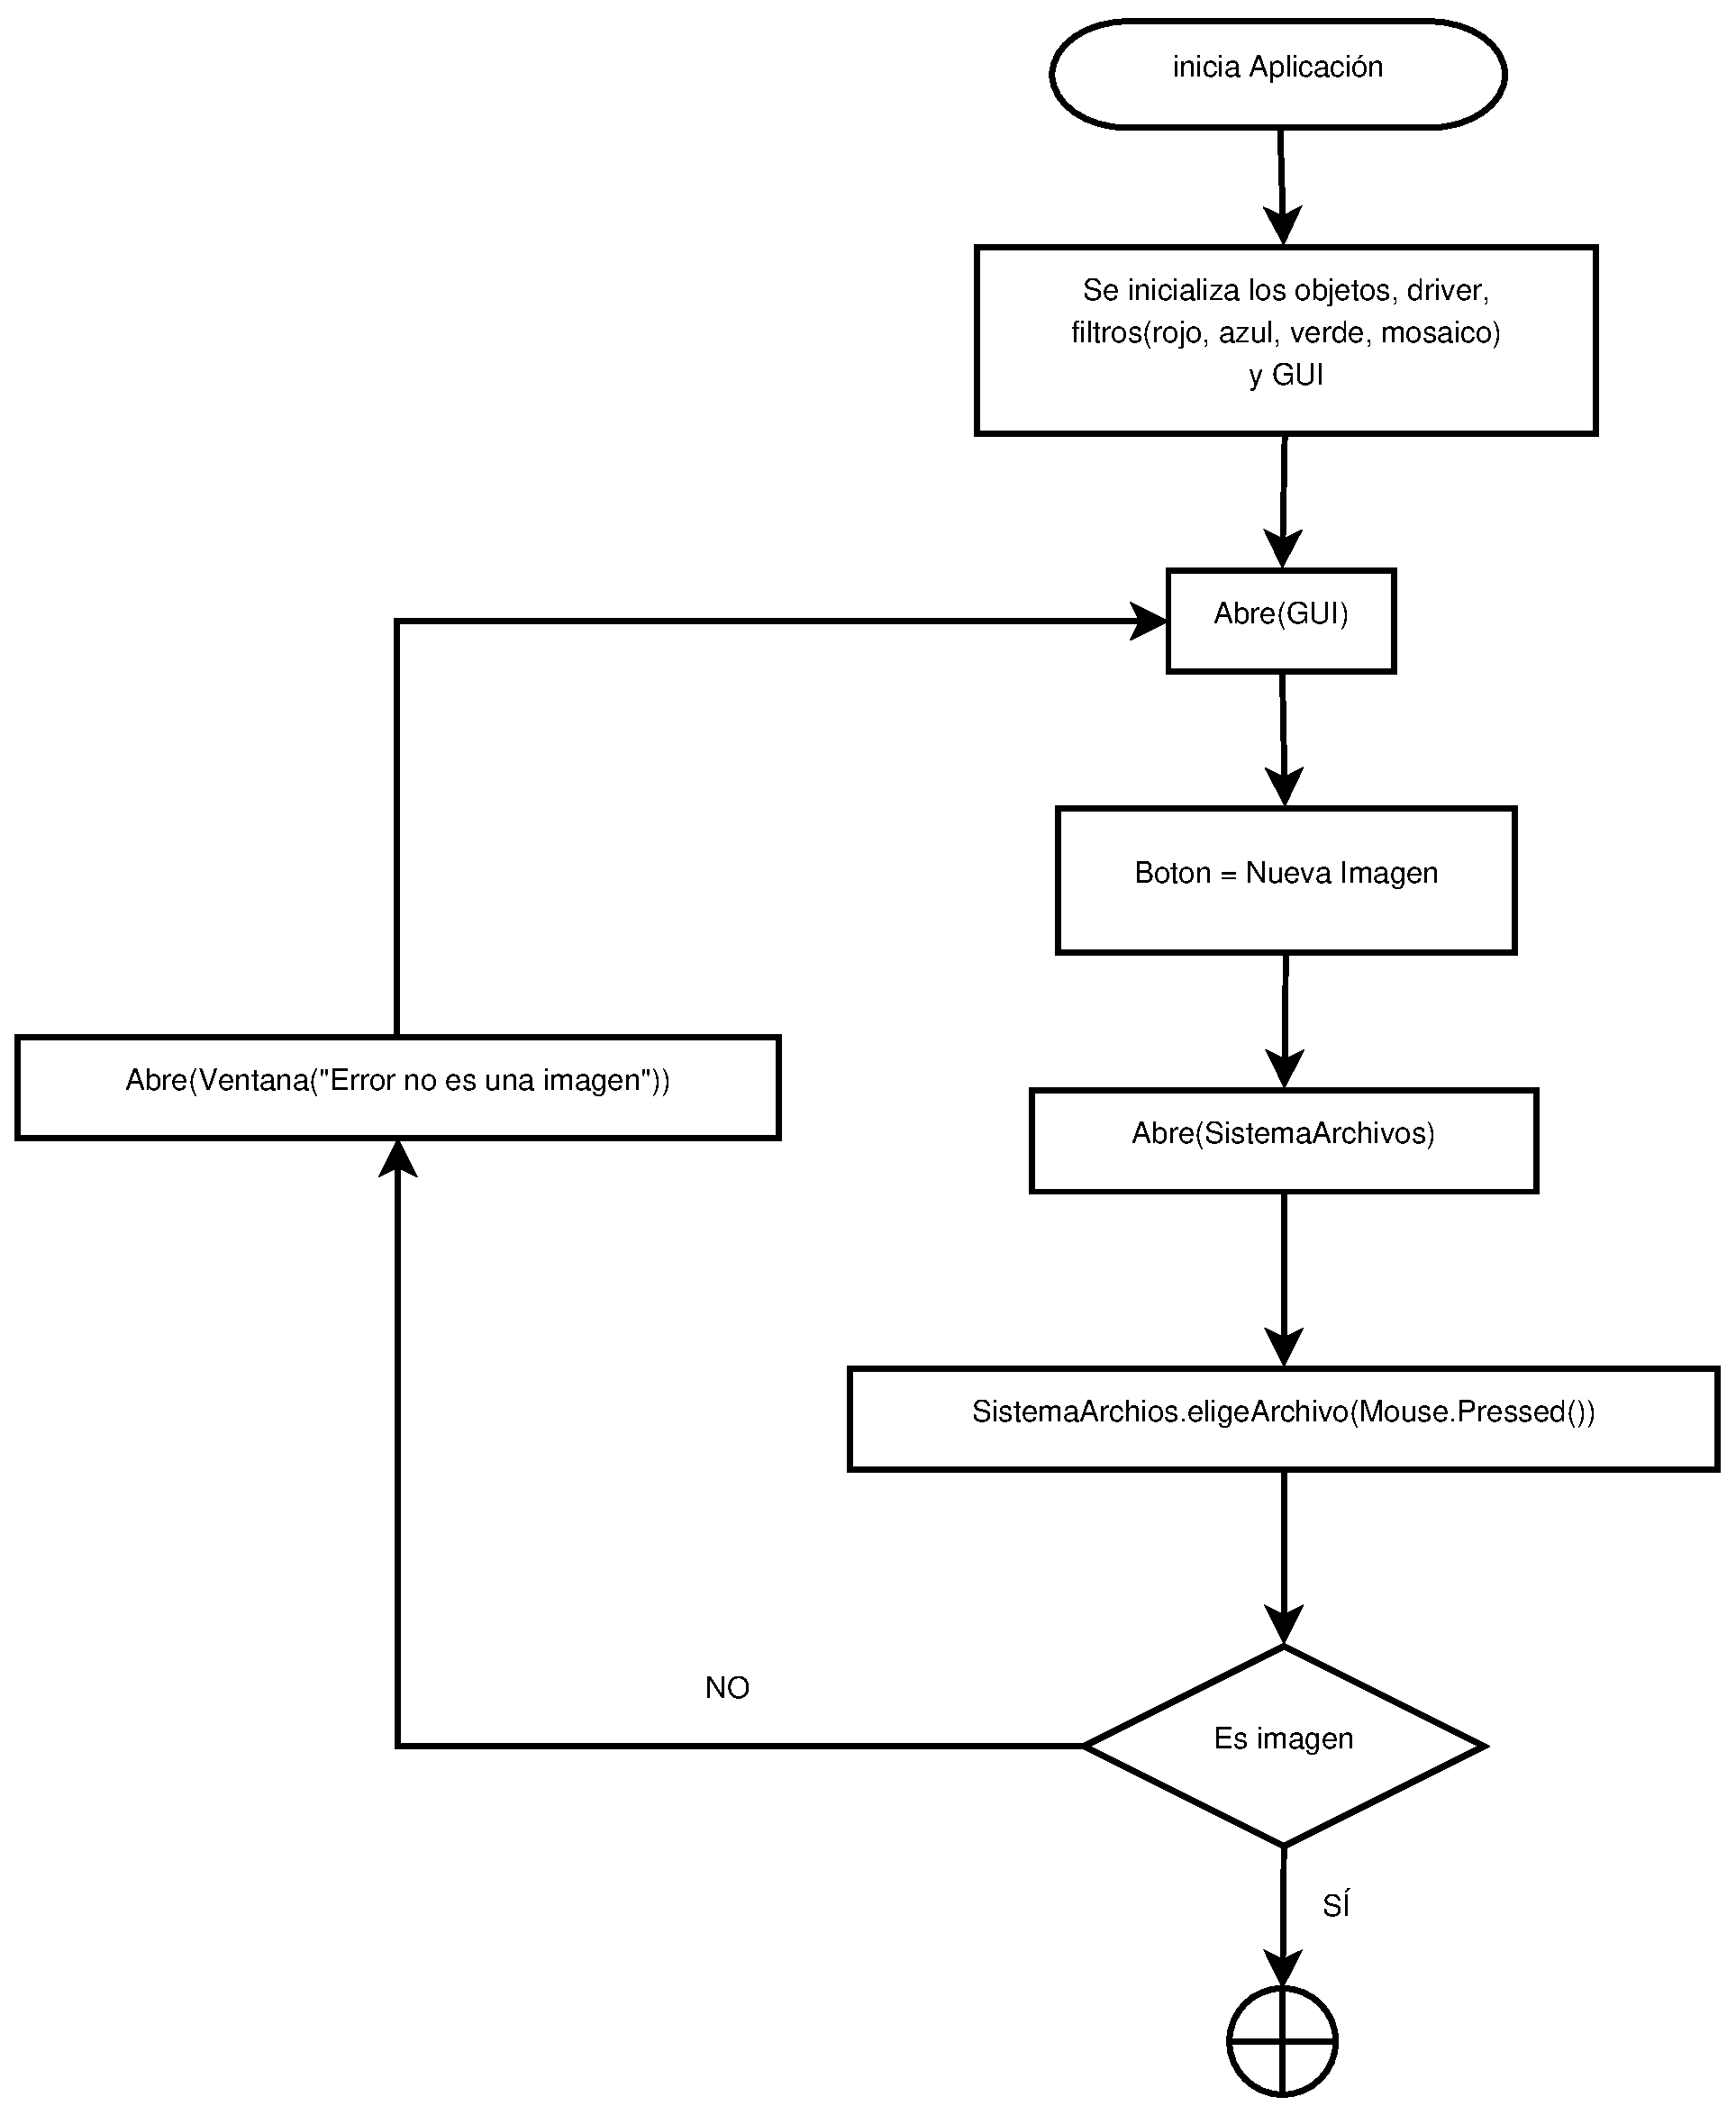
\includegraphics[scale=.36]{images/Diagrama1.eps} 
    \caption{Diagrama de Flujo,parte1}
\end{figure}
\begin{figure}[h]
    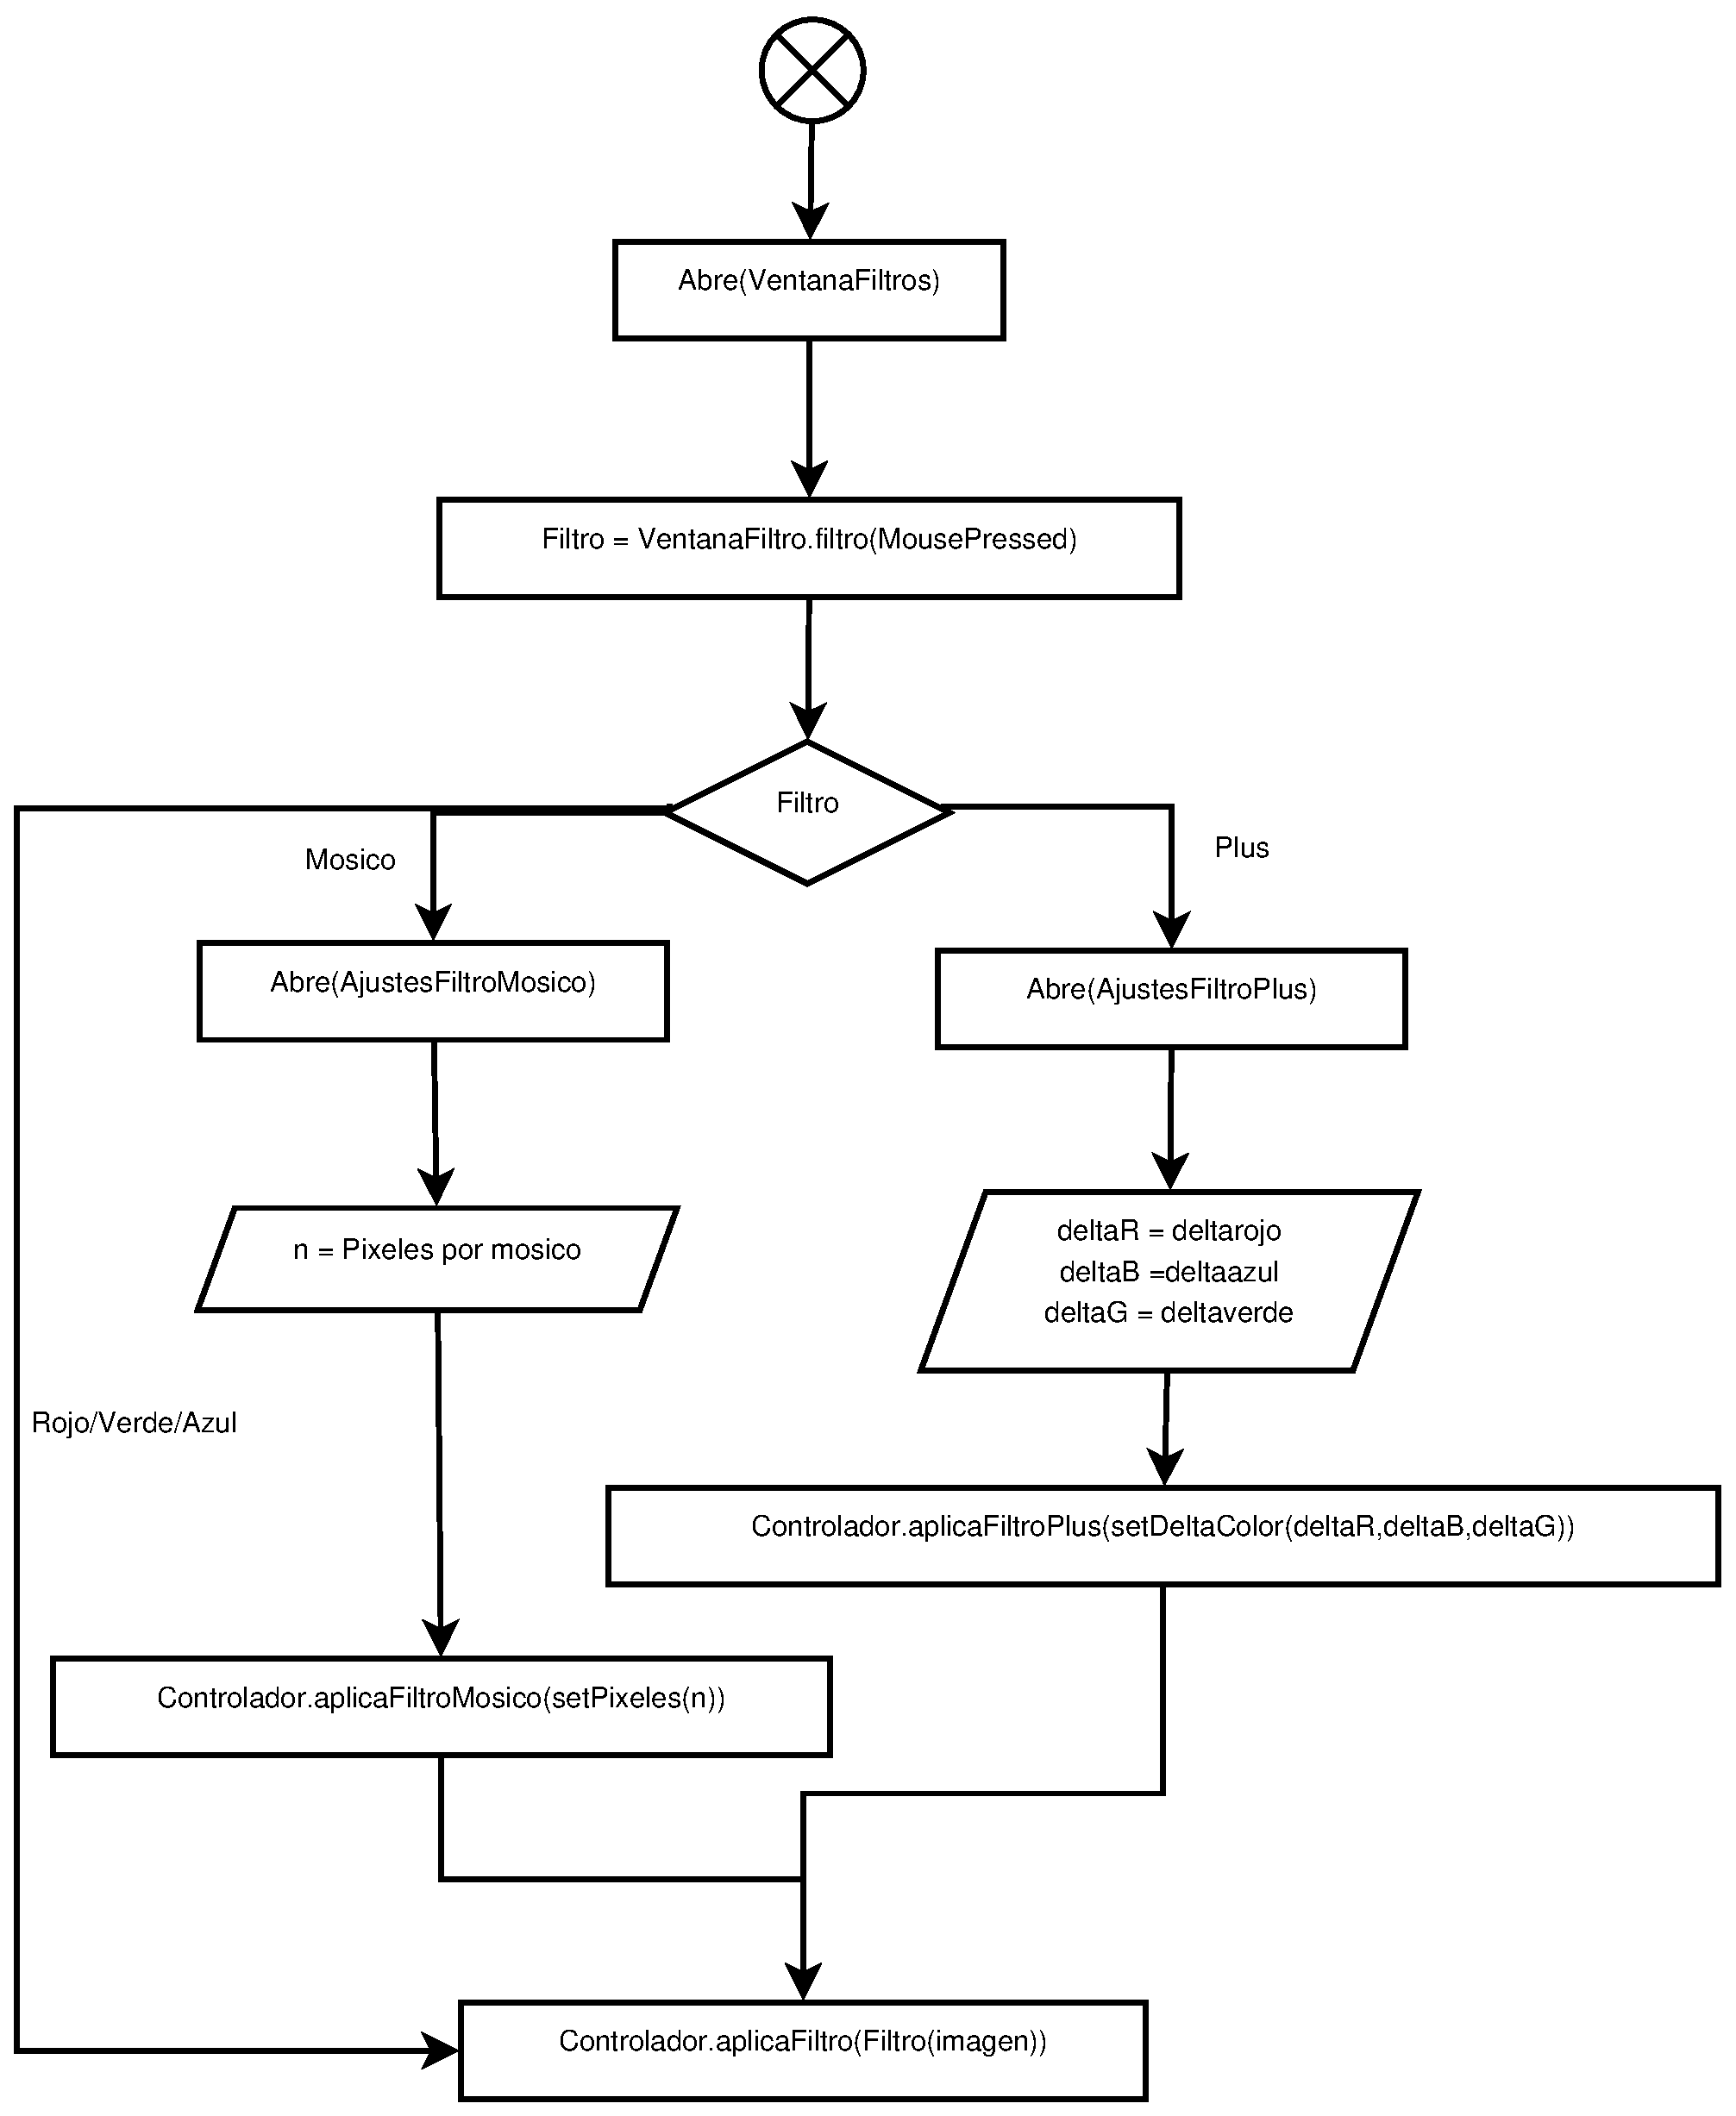
\includegraphics[scale=.42]{images/Diagrama2.eps} 
    \caption{Diagrama de Flujo,parte2}
\end{figure}
\begin{figure}[t]
    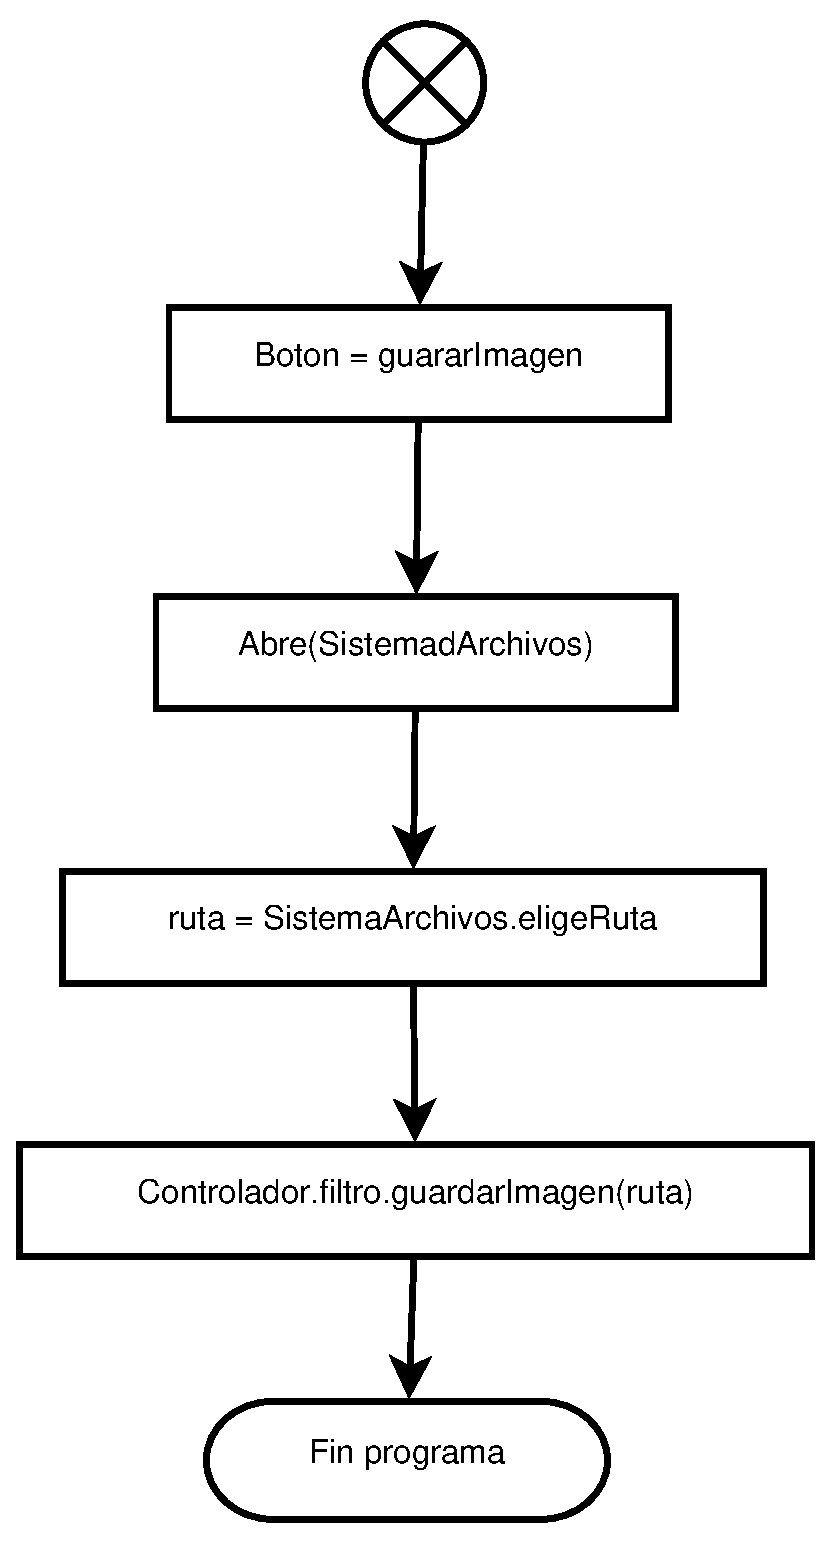
\includegraphics[scale=.73]{images/Diagrama3.eps} 
    \caption{Diagrama de Flujo,parte3}
\end{figure}
\end{document}